% -*- coding: utf-8-unix; mode: latex; fill-column: 70 -*-

\documentclass[bibtex,pagenumbers]{stabs2021}

% Leave option pagenumbers in to print page numbers in the header.
% This is helpful when writing the article and to facilitate review.
% Remove the option for final upload after acceptance.

% Use either option bibtex (default) or biblatex (recommended) to
% indicate the bibliography system you're using. See bibliography
% commands in the preamble and at the end of this file, and BibLaTeX
% and Biber documentation on CTAN: ctan.org/pkg/biblatex, ctan.org/
% pkg/biber.

% The class is based on the KOMA-Script article class and provides
% therefore all the features that that class provides. Documentation
% on CTAN: ctan.org/pkg/scrartcl.

% The following packages are loaded by the class and are therefore
% available without user intervention: babel, graphicx, hyperref,
% enumerate, booktabs, natbib (if bibtex), biblatex (if biblatex),
% censor, amsmath, and every symbol that amssymb defines.
% Documentation on CTAN: ctan.org/pkg/<pkgname>.

% Select your dialect of English for correct hyphenation patterns:
% see list of languages in documentation on ctan.org/pkg/babel,
% section 1.27 "Languages supported by babel with ldf files"
\selectlanguage{british}

% Uncomment following line if using BibLaTeX (recommended)
% See also \printbibliography at the end of this file
% \addbibresource{biblatex.bib}

\title{Guidelines for Preparation of Manuscripts}

% Uncomment following line to stop anonymizing the output
% Beware that \censor doesn't work across lines
% \StopCensoring
\author{
  \censor{Firstname Surname}, \censor{\textit{Affiliation}},
  \censor{\href{mailto:test@example.com}{test@example.com}}
  \and
  \censor{Firstname Surname}, \censor{\textit{Other affiliation}},
  \censor{\href{mailto:test@example.com}{test@example.com}}
}

\begin{stabsabstract}
  Authors of papers have to type these in a form suitable for direct
  photographic reproduction by the publisher. In order to ensure
  uniform style throughout the volume, all the papers have to be
  prepared strictly according to the instructions set below, which
  essentially follow the ITTC format.

  The abstract should be a brief description of the scope of the
  paper, not exceeding 100 words in length.
\end{stabsabstract}

\keywords{at least 3 suitable keywords for indexing purposes}

\begin{document}

% This command typesets the title, author, abstract, and keywords in
% one-column mode. Don't write out any text before it, as it would
% cause LaTeX to start a new page to break out of two-column mode.
\makestabstitle

\section{Introduction}

Please note that this section and all subsequent sections and
subsections are numbered. All main headings and sub-headings should be
typed in bold as shown below.

\section{Introductory Information for Authors}

\subsection{Word Processor}

It is highly recommended to generate the paper on a personal computer
or workstation using a recent version of the Microsoft Word program.
Other computers and word processing programs may be used, although in
this case, additional work by the proceedings editor is required on
the source file, in order to convert it to the present format.

\subsection{Digital Copy}

Authors should upload their papers through the ``Submit'' page of the
STAB\&S 2021 Conference web site (\href%
{http://www.stability-and-safety-2021.org/}%
{http://www.stability-and-safety-2021.org/}). Log in to the
conference's paper submission system and select ``Your Submissions''.

The maximum paper length, after formatting to the STAB\&S 2021
specification, is 10 pages. Whilst slightly longer papers can still be
accommodated, authors are advised to do their best in order to respect
this page limit.

\subsection{Liability}

Authors are responsible for obtaining security approval for
publication from employers or authorities, where necessary. If they so
wish, authors should include a disclaimer at the end of the paper
stating that the opinions expressed are those of the author and not
those of the company or organization that they are representing.

\section{Page Format}

It is required that the papers be prepared on \emph{A4 page} format
(210~mm \(\times\) 297~mm). All dimensions concerning the page layout
are given in millimetres. The Microsoft Word program allows the user
to specify the configuration using these metric dimensions.

\subsection{Top and Bottom Margins}

\paragraph{General.}

The bottom margin for all pages is 20~mm. This is the distance between
the \emph{bottom of the last line of text} and the \emph{bottom edge
of the sheet of paper}. The top margin for all pages is 32~mm. The top
margin is measured from the \emph{top edge of the paper} to the
\emph{top of the first line of text}.

\subsection{Columns and Side Margins}

The manuscript is required to be prepared in two-column format. The
column width is to be 81~mm and the spacing between the columns is to
be 8~mm. The left side margin is to be 20~mm. The corresponding right
hand margin is 20~mm.

\section{Manuscript Format Conventions}

\paragraph{Font.}

The text font must be 12~point ``Times New Roman'' type (the most
common type fonts available on laser printers). Greek letters
appearing in equations or text (such as \(\alpha\), \(\beta\),
\(\gamma\)) should also be 12~point and set in the standard ``Symbol''
type font. The vertical line spacing should be 14~points (equating a
line height of 4.95~mm).

\paragraph{Justification.}

The text (but not the headings) should also be justified so that it
fills up the space in the columns exactly. Hyphenation (a standard
feature on most word processors) should be used to break the text so
that it nearly fills each line. The appearance of the volume will be
compromised if the text has not been hyphenated, since justification
can lead to some lines with large spaces between the words.

\paragraph{Paragraphs.}

All paragraphs are to be indented 6~mm. Paragraphs should not be
separated from any blank line. The proper distance between paragraphs
(14~pt) is to be assigned through the properties of the paragraph
itself.

All features described in the three paragraphs above are automatically
implemented in typing text using the ``Paragraph-1'' style included in
the present format file.

\subsection{Headings}

Headings and subheadings should appear throughout the paper to divide
the subject matter into logical parts and to emphasize the major
elements and considerations. Each section may have subheadings, as
detailed below. Parts or sections should be numbered with one digit
(X.) for the main headings, two digits (X.X) for the first
subheadings. Further subheadings should not be numbered.

Headings should not appear at the bottom of a column, if there is no
text following them in the same column. If the normal flow of text
causes this to occur, the editor may try to prevent it by formatting
one or more neighbouring paragraphs with ``Paragraph-1+'' so that the
heading appears at the top of the next column.

\paragraph{Major Headings.}

Major headings should appear in bold capital letters and aligned flush
with the left-hand margin of the column. Space corresponding to two
blank lines should be left above the major heading and to one blank
line below it. All these features are automatically implemented if the
``Major-Heading'' style is used, which is included in the present
format file. The only exception to the standard format for major
headings is represented by the first major heading located at the top
of the left column in the first page (``INTRODUCTION'' in the present
sample file), for which the ``Major-Heading-Top'' style is used, to
avoid leaving at the column top the space corresponding to the two
blank lines.

\paragraph{Subheadings.}

Subheadings should appear in bold letters with the initial letter of
each word capitalized and aligned flush with the left-hand margin of
the column. Space corresponding to two blank lines should be left
above the major heading and to one blank line below it. All these
features (apart from typing capitalised initial letters for each word)
are automatically implemented if the ``Subheading'' style is used,
which is included in the present format file. The only exception to
the standard format for subheadings is represented by a subheading
that may happen to be located at the top of the right column in the
first page. In this case the ``Subheading-Top'' style can be used, to
avoid leaving at the column top the space corresponding to the two
blank lines.

\paragraph{Sub-Subheadings.}

Sub-subheadings should be indented 6~mm and appear in underlined
letters, with the initial letter of each word capitalised. The
sub-subheading should be followed by a period, two spaces and the
text. One line of space should be left above the sub-subheading. All
these features (apart from typing capitalised initial letters for each
word) are automatically implemented if the ``Subheading'' style is
used, which is included in the present format file.

\subsection{Footnotes}

Footnotes are references with superscript numerals and are to be
numbered consecutively from 1 to the end of the
paper\footnote{Footnotes should appear in ``Times New Roman'' font in
the smaller 10~point type.}. Footnotes should appear at the bottom of
the column in which they are referenced or, if necessary, at the
bottom of the next column on the same page. A solid line is used in
this format to separate the footnotes from the rest of the
text\footnote{The line above the footnote is optional, but it does
help to keep the footnotes separate from the main body of text}.
Whenever possible, the use of footnotes should be avoided.

\subsection{Tabulations/Enumerations}

Where several considerations, conditions, requirements, or other
qualifying items are involved in a presentation, it is often
advantageous to put them in tabular or enumerative form, rather than
to run them into the text. This arrangement, in addition to
emphasizing the items, creates a graphic impression that aids the
reader in accessing the information and in forming an overall picture.
It is customary to identify the individual items as:
\begin{enumerate}[(1)]
  \item First,
  \item Second,
  \item Third,
\end{enumerate}
or:
\begin{enumerate}[(a)]
  \item First,
  \item Second,
  \item Third,
\end{enumerate}
or simply using bullets:
\begin{itemize}
  \item First,
  \item Second,
  \item Third.
\end{itemize}
The above arrangements can be obtained in this format using the
``Numbered-1'', ``Lettered-1'' and ``Pointed-1'' styles, respectively.
Although inclusion of such elements makes the text livelier, care
should be taken not to use this scheme too frequently, as it can make
the reading choppy and invalidate their purpose and usefulness.

Tables can also be included, see table~\ref{tbl:example-table} for an
example.

\begin{table}[ht]
  \centering
  \caption{Avoid using vertical lines and use thicker horizontal lines
    above and below the table.}
  \label{tbl:example-table}
  \begin{tabular}[t]{lcc}
    \toprule
    & Treatment A & Treatment B \\
    \midrule
    John Smith   &  1 & 2 \\
    Jane Doe     & -- & 3 \\
    Mary Johnson &  4 & 5 \\
    \bottomrule
  \end{tabular}
\end{table}

\section{Mathematics}

Equations should be numbered consecutively beginning
with~\eqref{eq:bernoulli} to the end of the report, including any
appendices. The number should be enclosed in parentheses (as shown
above) and set flush right in the column on the same line as the first
line of the equation. This is the number that should be used when
referring to equations within the text.

\subsection{Printing}

Equations should be typed using the standard equation editor available
on Microsoft Word program. Vector quantities should appear in bold
lower case letters and tensor quantities in bold upper case letters.
For instance, the Bernoulli equation is:
\begin{equation}
  \label{eq:bernoulli}
  \frac{\partial\phi}{\partial t}
  + \frac{1}{2} \lvert \nabla \phi \rvert^2 + \frac{P}{\rho} + g y
  = C(t)
\end{equation}

The continuity and Navier-Stokes equations are:
\begin{gather}
  \nabla \cdot \vec{u} = 0 \\
  \frac{\partial \vec{u}}{\partial t} + \vec{u} \cdot \nabla \vec{u}
  = -\frac{1}{\rho} \nabla p - \vec{g} + \nu \nabla^2 \vec{u}
\end{gather}

In all mathematical expressions and analyses, any symbols (and the
units in which they are used) not previously defined in the
nomenclature should be explained. An extra line of space is to be left
above and below a displayed equation or formula. To achieve this, in
the present format the equations have been included in tables, so that
blank table rows can be exploited. However, this is just a suggestion,
and different techniques can be used.

\section{Graphic Material}

\subsection{General Guidelines}

All figures (graphs, line drawings, photographs, etc.) should be
numbered consecutively and have a caption consistent of the figure
number and a brief title (the ``Figure-Cap'' style can be used to
automatically number the figures, as shown by the example). This will
also allow automatic referencing of the figure within text. Many
different file formats are accepted (or created) by Microsoft Word, to
be inserted and formatted along with text.

All illustrations should be clearly referenced in the text; these
should be placed in the main body of the text.

Figures should be produced electronically in e.g. .jpg, .png, or .tiff
formats. Save another copy of each individual graphic in separate
files (Fig1, Fig2, etc.) in addition to the complete manuscript file.
The resolution should be at least 300dpi, and preferably above 500dpi.
Thin line computer prints of curves, etc. must be thickened. Figures
may be in colour or in black and white. Please note that the hardcopy
version of the proceedings will be printed in black only. If you use
colour graphics please check the graphic in black and white to see if
shading or hatching is needed.

\subsection{Placement}

Depending on size, the artwork, graphs, charts, line drawings,
sketches and diagrams, etc. should be positioned either within one
column or spanning both columns (in this case, a frame should be used
to include the figure or table and the caption, similar to that used
for the paper title). If the figure spans two columns, the caption
should be properly centred (the ``Figure-Cap-C'' style may be used in
this case). Captions for figures are placed below the figures while
table captions (``Table-Cap'' and ``Table-Cap-C'' may be used for the
case of Justified and Centred Captions, respectively) are placed above
the tables. Space corresponding to a blank line should be provided
above and below figures and their captions.

\subsection{Example}

Figure~\ref{fig:example-figure} is an example of how a figure used in
a single column should be arranged on the page.

\begin{figure}[ht]
  \centering
  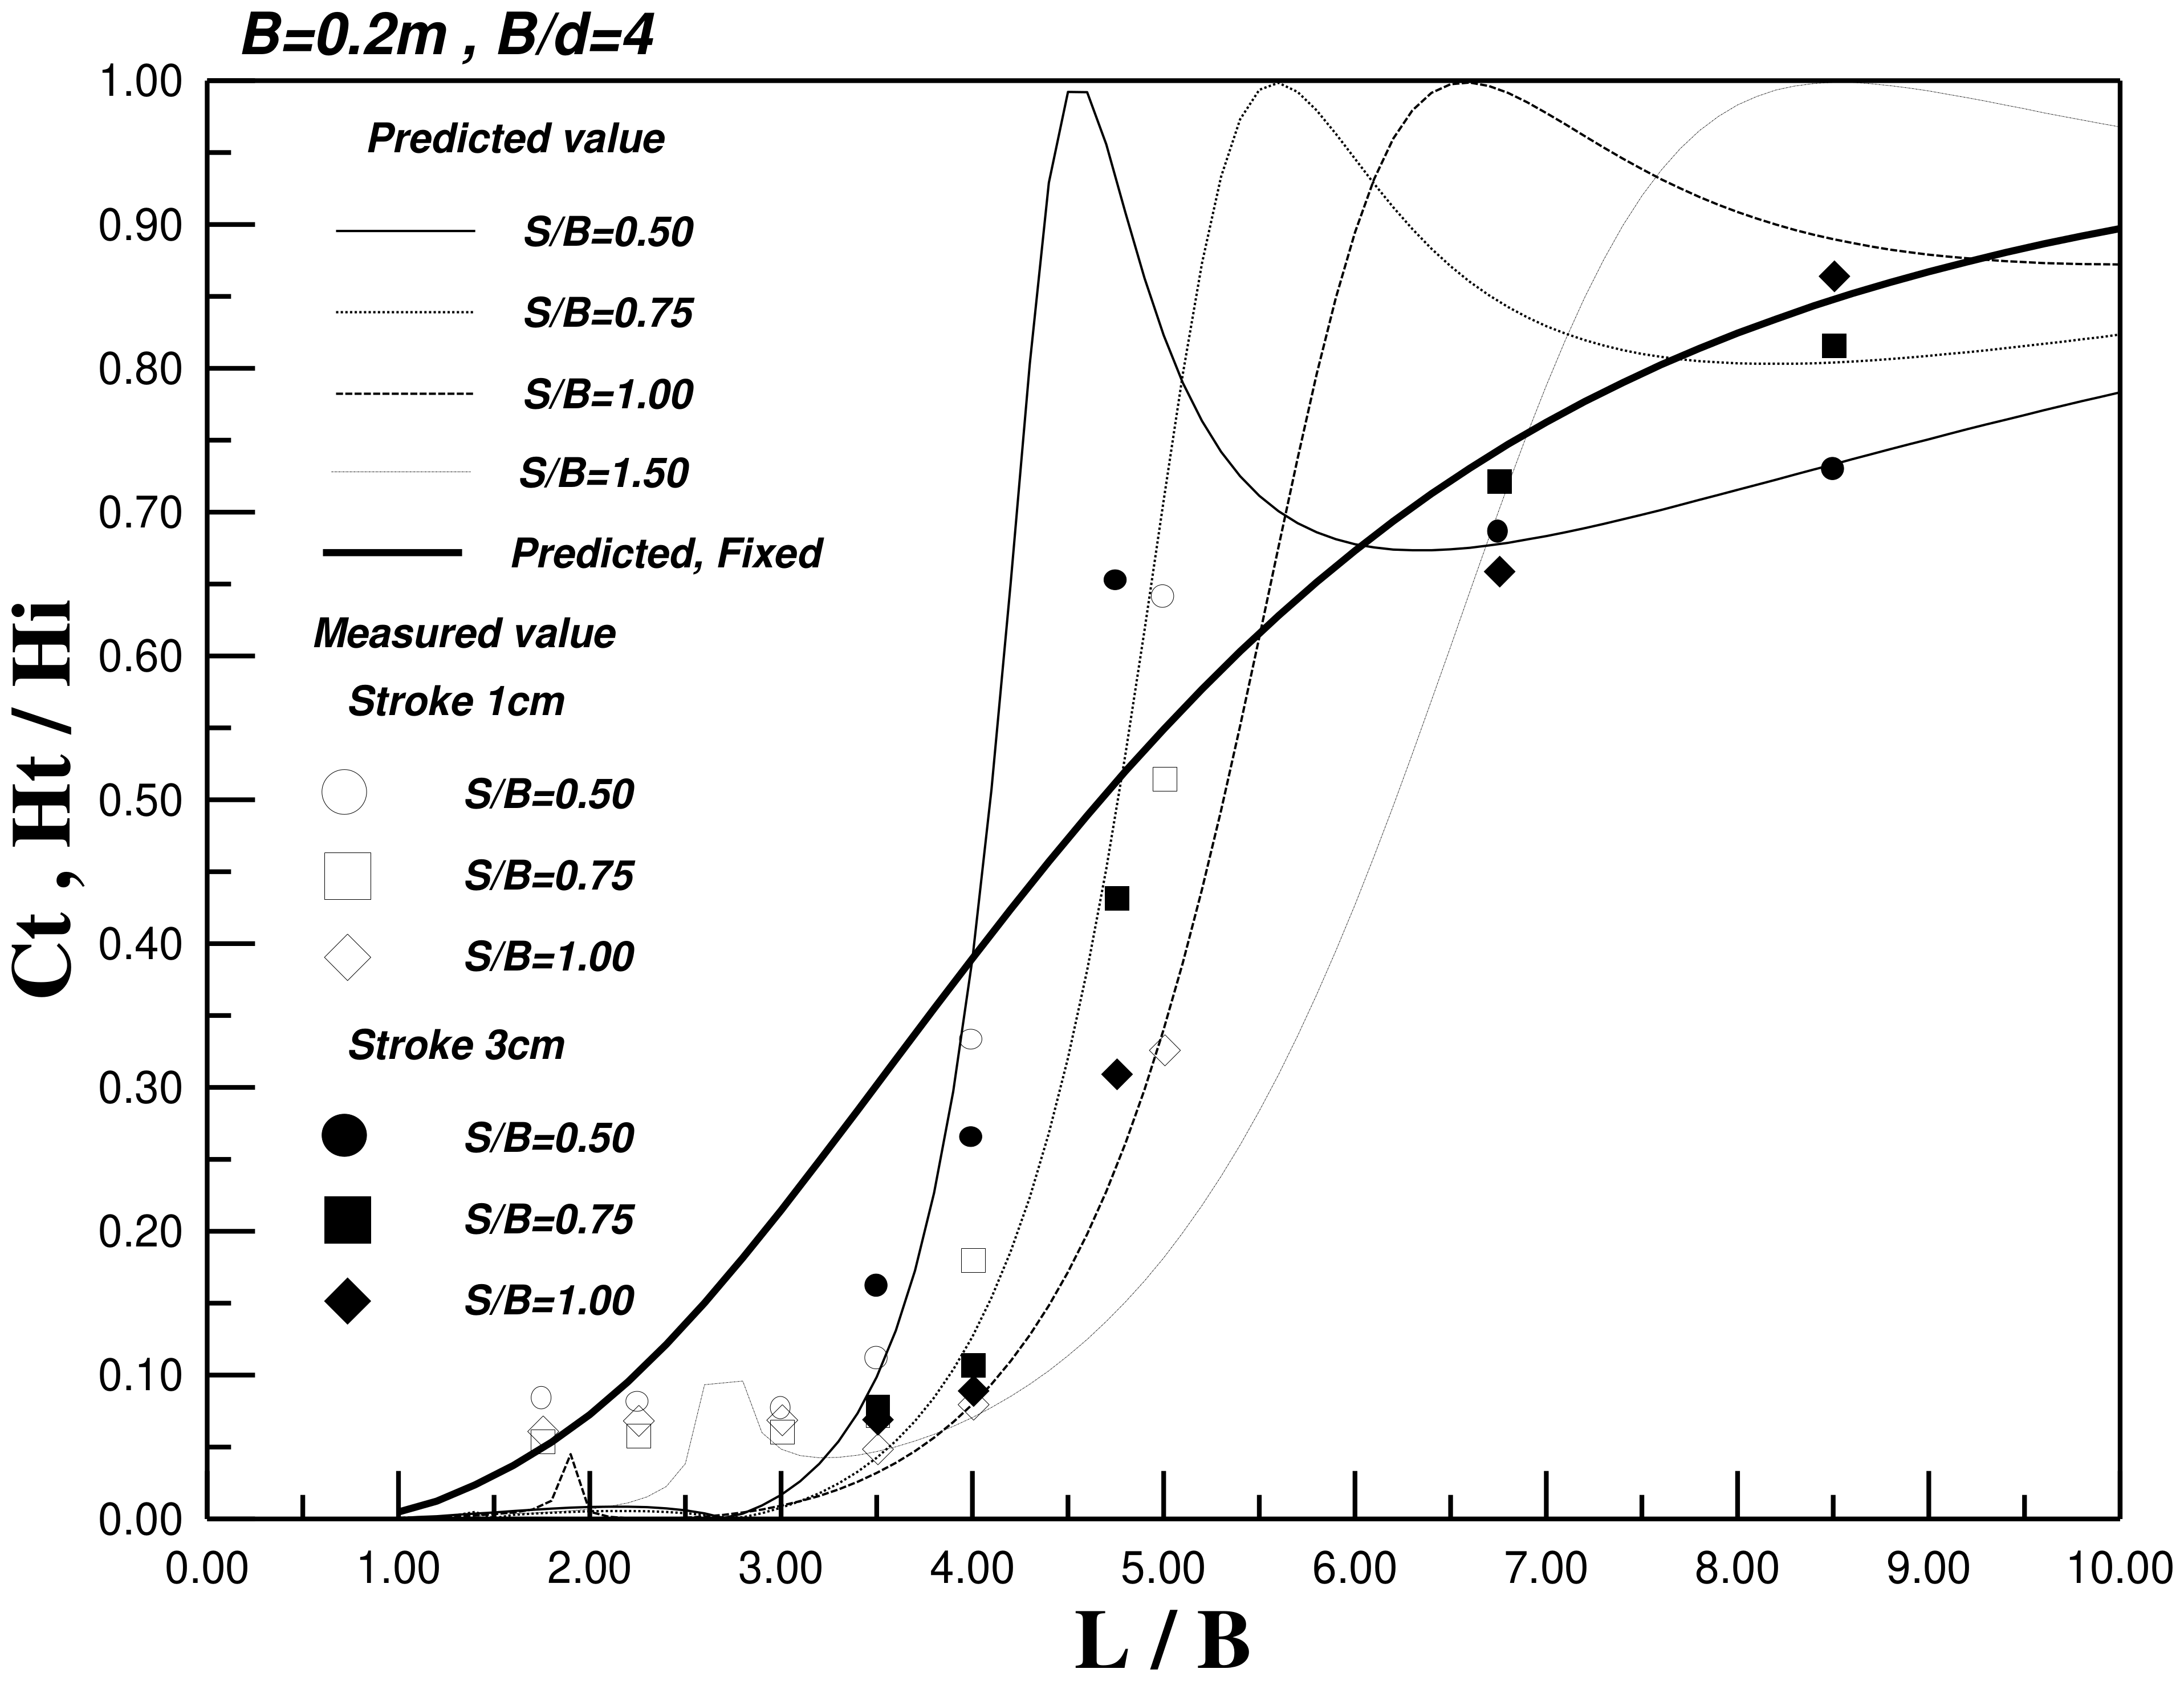
\includegraphics[width=\linewidth]{stabsgraph.png}
  \caption{Transmission coefficient vs. \(L/B\) with separation
    distance variation. \(B = 0.2~\mathrm{m}\), \(B/d = 4\).}
  \label{fig:example-figure}
\end{figure}

\subsection{Lettering}

For good legibility, lettering (call-outs) in figures must be 2~mm
high or higher on the material as it is placed on final report.

Lettering may be in any appropriate font, although common sans serif
fonts (such as Helvetica) often look best on charts and graphs.

\section{Conclusions}

The main body of the text should end with the conclusions of the
paper.

\section{Acknowledgments}

Brief acknowledgments may be added.

\section{References}

\subsection{Text Citation}

Within the text, references should be cited by giving the last name of
the author(s) and the year of publication of the reference. The year
should always be enclosed by parentheses, while enclosing the name of
the author(s) within the same parentheses depends on the context. Some
examples using the sample references listed below are illustrated
hereafter:

% If using BibTeX (default), use natbib's \citet and \citep commands
% for textual and parenthetical citations, respectively.

% If using BibLaTeX (recommended), use the package's \textcite and
% \parencite commands instead. The stabs2021 class loads BibLaTeX
% with the option natbib=true so that natbib's citation commands may
% still be used.

\dots\ It was shown by \citet{kwon1981prediction} that numerical
integration of the Navier-Stokes equations can be successfully
performed for low Reynolds numbers. \dots

\dots\ Heat transfer in a duct is improved substantially by using
small, rectangular protuberances \citep{sparrow1980forced}. \dots

\dots\ Convection of this type is treated in several sources
\citep{lee1982structure, sparrow1980fluid, tung1982evaporative}. \dots

\subsection{List of References}

References for cited material should be listed at the end of the
report. They should be arranged in alphabetic order according to the
last name of the (first) author. Each reference should include the
last name of each author followed by the authors' initials, and typed
with the first line aligned flush left; the second and the subsequent
lines are indented 6~mm (``Reference style'' can be used).

\subsection{Journal References}

These references (as well as papers in conference proceedings, or any
other collection of works by numerous authors) should include:
\begin{itemize}
  \item The year of publication,
  \item The full title of the cited article,
  \item The full name of the publication in which it appeared,
  \item The volume number, edition number and page numbers.
\end{itemize}

\subsection{Books}

References to books (including textbooks, monographs, theses and
technical reports) should include:
\begin{itemize}
  \item The year of publication,
  \item The full title of the cited article,
  \item The publisher,
  \item The inclusive page numbers of the work being cited.
\end{itemize}

In all cases, titles of books, periodicals and conference proceedings
should be in italics. A sample list of references in which these forms
are illustrated is shown hereafter.

% Uncomment following line if using BibTeX (default)
\bibliography{bibtex}

% Uncomment following line if using BibLaTeX (recommended)
% See also \addbibresource{biblatex.bib} in the preamble
% \printbibliography

\appendix

\section{Appendix}

Put appendices, if any, after the bibliography.

\end{document}
